%%%%%%%%%%%%%%%%%%%%%%%%%%%%%%%%%%%%%%%%%%%%%%%%%%%%%%%%%%%%%%%%%%%%%%%%%%%%%%%%
%2345678901234567890123456789012345678901234567890123456789012345678901234567890
%        1         2         3         4         5         6         7         8

\documentclass[conference]{ieeeconf}
%\usepackage{times}

% Subfiles package
%\usepackage{subfiles}

% References
%\usepackage[numbers]{natbib}

% Usual setup packages
\usepackage{listings} % For including source code with highlighting
\usepackage{hyperref} % For better hyper-link integration
\usepackage[bottom]{footmisc} % places footnotes at page bottom

% Packages for verbatim text blocks
\usepackage{alltt} % Package for including math in verbatim text
\usepackage{fancyvrb}

% Packages for math symbols and other mathey things
%\usepackage{amsthm}
\newtheorem{theorem}{Theorem}
\newtheorem{claim}{Claim}
\newtheorem{corollary}{Corollary}
\newtheorem{proposition}{Proposition}
\usepackage{amsmath}
\usepackage{amsfonts}
\usepackage{amssymb}

% Packages for including pseudo-code
\usepackage{algorithmicx}
\usepackage{algorithm}
\usepackage{algpseudocode}

% Packages that handle tables, figures and other floats
\usepackage{enumerate}
\usepackage{tabularx}
\usepackage{multirow}
\usepackage{float} % To make floats movable
\usepackage{subcaption}
\usepackage[table]{xcolor}

% Packages for drawing graphs, FSMs, etc.
\usepackage{pgf}
\usepackage{tikz}
\usetikzlibrary{shapes,arrows,calc,fit,positioning,shapes.symbols,shapes.callouts,patterns,automata,matrix}

% Remove red boxes around refs
\hypersetup{
    colorlinks,
    citecolor=black,
    filecolor=black,
    linkcolor=black,
    urlcolor=blue
}

% ------------------------------ CUSTOM MACROS ------------------------------------
% Nice little macro for adding a comment box. Include incrementing comment numbers.
\newcounter{comcount}
\setcounter{comcount}{0}
\newcommand{\mycomment}[1]
{
\refstepcounter{comcount}
\smallskip\noindent\fbox{\parbox{\linewidth}{\emph{Comment \arabic{comcount}} : \small{#1}}} 
}

\DeclareMathOperator*{\argmin}{\arg\!\min\>}
\newcommand{\amin}[1]{\underset{#1}\argmin}
\DeclareMathOperator*{\argmax}{\arg\!\min\>}
\newcommand{\amax}[1]{\underset{#1}\argmax}

\def\a{\mathbf{a}}
\def\Z{\mathbb{Z}}
\def\R{\mathbb{R}}
\def\N{\mathcal{N}}
\def\estt{\hat{\tau}}
\def\estg{\gamma}
\newcommand{\sig}{\mathcal{S}}
\newcommand{\ceil}[1]{\lceil#1\rceil}
\newcommand{\xm}{x_{\hat{m}}}

\begin{document}
\title{Modeling Collaborative Swarming Behavior as a Global Game}
\author{Author Names Omitted for Anonymous Review. Paper-ID [add your ID here]}

\maketitle

%%%%%%%%%%%%%%%%%%%%%%%%%%%%%%%%%%%%%%%%%%%%%%%%%%%%%%%%%%%%%%%%%%%%%%%%%%%%%%%%
\begin{abstract}
Abstract goes here\ldots
\end{abstract}

\IEEEpeerreviewmaketitle

%%%%%%%%%%%%%%%%%%%%%%%%%%%%%%%%%%%%%%%%%%%%%%%%%%%%%%%%%%%%%%%%%%%%%%%%%%%%%%%%
\section{Introduction}\label{sec:intro}
Collaborative tasks are an important set of scenarios often studied in the field of swarm robotics. Many of the tasks we envision teams of robots performing, such as object transport \cite{sugawara2012}, oil-spill containment \cite{beni2005swarm}, firefighting \cite{krishnanand2006glowworm}, pattern recognition  \cite{beni1993swarm}, and cooperative surveillance fall under this broad umbrella of collaborative tasks. While considerable work has been done in studying the specific details of particular tasks in the above list, the more general question of estimating a team size appropriate for the size of the task remains largely unanswered. It is generally assumed that a required team size is provided by a domain expert before a collaborative task is attempted by the robots. But, as is often the case with teams of humans attempting a collaborative task, this number not easy to guess, e.g., When trying to lift and move a heavy object, it is difficult to estimate how many people will be required. A number of factors such as the mass and dimensions of the object, and the length and complexity of the path (perhaps involving staircases) come into play when deciding this number. Therefore, there exist a range of team sizes that may accomplish this task to varying degrees of success.

\begin{figure*}[!ht]
\centering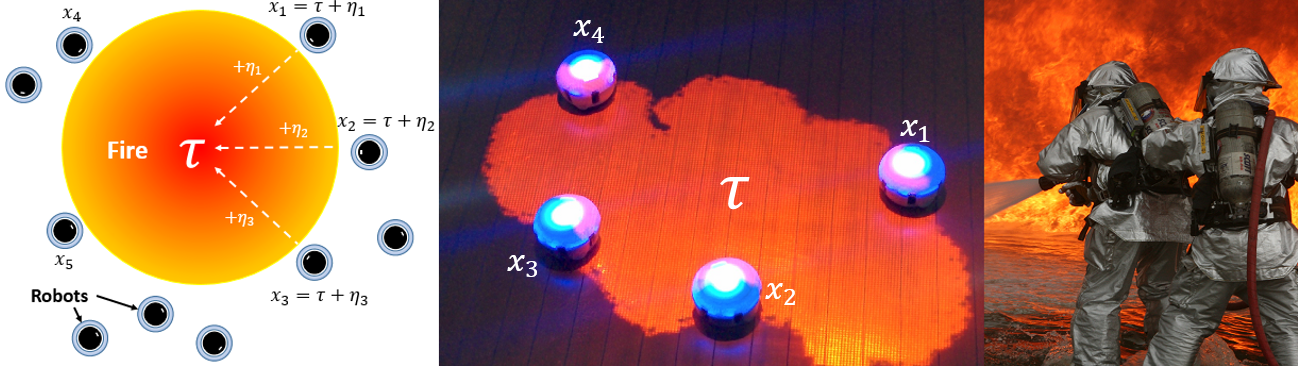
\includegraphics[width=\textwidth]{../figures/dropletfire.png}
\centering\caption{}\label{fig:dropletfire}
\end{figure*}

The goal of this paper is to model and analyze such tasks that have the property of \emph{concurrent benefit} using the concept of global games from the field of game theory. We define concurrent benefit as an attribute of a collaborative task wherein the exact number of agents required to successfully complete the task is unknown and varies with time. The probability of success depends, non-linearly, on the average number of agents assigned to that task. For example, in a firefighting scenario (see Fig.~\ref{fig:dropletfire}), a single robot trying to contain a large fire will likely be unsuccessful on its own (and will waste fire retardant in trying) but a group of robots within a certain group size range may be able to contain the flames to a reasonable level of success. This measure of success is related non-linearly to the group size, i.e. where 5 or even 10 robots have a negligible effect on containing the fire, perhaps 12 or more very quickly become capable of succeeding in the task.

Collaborative tasks can be modeled as a global game with multiple players/agents. All tasks take place in a large operational area. Tasks or collaboration sites appear within the operational area at random. All agents are dispersed uniformly and at random within the operational area. The reader should note that the method of searching for a collaboration site is arbitrarily chosen for the purposes of the model discussed in this paper; in practice, any search pattern or algorithm that best fits the scenario may be chosen without affecting the conclusions provided by our model. Once an agent arrives at a collaboration site, it independently makes an estimate, $\tau$, for the group size required to successfully complete the task at that site. This estimate is derived from an estimation function, $\Xi(\cdot)$, that takes in a noisy signal, $x$, as input. $\Xi(x)$ quantifies the size and complexity of the presented task using the robot's sensors and internal state information. This is analogous to a human assessing a situation using their senses and other domain specific data provided to him. The reason for using an estimation function is discussed in Section\ref{sec:ggresults} of this paper.

\begin{figure}[!ht]
\centering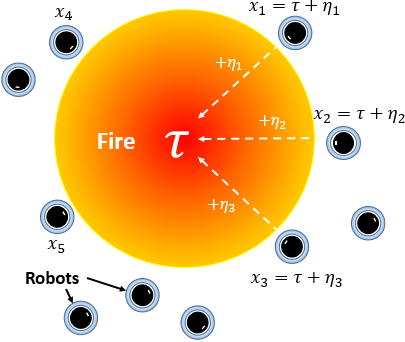
\includegraphics[width=.75\columnwidth]{../figures/globalgamesetup.png}
\centering\caption{}\label{fig:ggsetup}
\end{figure}

The noisy signal $x$ is a sum of two terms, $x = \theta + \epsilon$, where $\theta$ is considered the \emph{ground truth} signal and $\epsilon$ is a Gaussian noise term with mean $0$ and standard deviation $\sigma$, as seen in Fig.~\ref{fig:ggsetup}. This setup helps situate this multi-robot collaboration model in a global game setting. The \emph{player} terminology often used in game theory literature maps directly to robots (or agents) in swarm robotics. Each player/agent makes independent algorithmic decisions and overall system equilibrium conditions are measured via the set of joint actions between agents. A brief overview of the theory of global games is provided in Section \ref{sec:ggoverview}.

\subsection{Related Work}\label{subsec:rw}



\section{Global Games: A Brief Overview}\label{sec:ggoverview}
Game theory is the study of strategic interactions among multiple agents or players, such as robots, people, firms, etc. where the decision of each party affects the payoff of the rest. A fundamentally important class of games is one with incomplete information where each agent's utility depends not only on the actions of the other agents but also on an underlying fundamental signal that cannot be accurately ordained by the agents. Returning to our previous example of firefighting, this fundamental signal is the difficulty of the task of putting out the fire. The size and intensity of the fire, along with environmental and other site-specific factors all play a major role in determining whether an agent should begin the task or wait for more help to arrive. 
%As an example, consider the decision making problem where each  person is deciding whether use a given road today or not. The congestion of the given road not only depends on how many other people are using the road but also, the weather condition which is unknown to the people. Some people may use the weather forecast to gain more knowledge on this unknown parameter but regardless, the utility of each agent depends on the unknown fundamental of weather condition. 

This class of global games with incomplete information was originally introduced in \cite{Carlsson1993} where two players are playing a game and the utility of the two players depends on an underlying fundamental signal, $\theta$, but each agent observes a noisy variation of $\theta$. Note that noisy variation in $\theta$ is not a result of inaccuracy in sensor measurements but represents a culmination of underlying unknown factors of the scenario. We discuss how sensor noise, from agents measuring the fundamental signal, can be modeled in the following section. Global games have been substantially generalized to study and model different economical phenomena such as pricing debt, currency crisis, and bank runs. See \cite{Morris2000} and the references therein for more details.
%A subclass of games with incomplete information is the class of global games which was originally introduced in \cite{Carlsson1993} where two players are playing a game and the utility of the two players depends on an underlying economics fundamental $\theta$ and each agent observes a noisy variation of $\theta$. Such games have been substantially generalized to study and model different economical phenomena such as pricing debt, currency crisis, and bank runs, see \cite{Morris2000} and the references therein for more details.



\section{Concurrent Benefit Task with Incomplete Information}
In this section, we mathematically define a concurrent benefit task which is central to our study. Consider a set of $n$ robots and suppose that each robot has an action set $A_i=\{0,1\}$ where $0$ represents ``not participating'' in the task and $1$ represents ``participating'' in the task.  Another object which plays an important role in our formalism is the \textit{easiness} parameter $\theta$ of the given task. We let $\theta$ be an (often random) real number which simply represents how easy/hard a task is and we further assume that it belongs to an interval $E=[c,d]$ in $\R$.  Finally, we let $u_i:A_1\times\Z^+\times \R\to \R$ be the utility of the $i^{\text{th}}$ robot, where $u_i(a_i,g,\theta)$ is the utility of the $i^{\text{th}}$ robot when $g$ other robots have decided to participate in the task and $\theta$ is the easiness parameter of the task\footnote{In general, the utility of each robot depends on the joint actions of the rest of the robots. However, here we assume that the utility depends only on the number of robots participating in the activity. The following discussions can be substantially generalized to a more general setting but this form of utility serves the purpose of this study.}. 

We define a task $T$ to be a \textit{concurrent benefit task} if: 
\begin{enumerate}[a.]
	\item $u_i(1,g,\theta)\geq u_i(0,g,\theta)$ for all $g\in[n-1]:=\{0,1,\ldots,n-1\}$ and $\theta \in E$. 
	\item $u_i(a_i,g,\theta)$ is an increasing and continuous function of $\theta$ for any $a_i$ and $g$. 
	\item $u_i(1,g,\theta)-u_i(0,g,\theta)\geq u_i(1,g',\theta)-u_i(0,g',\theta)$ for any $g\geq g'$ in $[n-1]$ and any $\theta\in E$. In other words, the more the number of the rest of the robots participating in the task, the more beneficial would be taking part in the activity.
	\item For any $g$ and any $\theta\geq \theta'$, we have $u_i(1,g,\theta)-u_i(0,g,\theta)\geq \lambda (\theta-\theta')$. 
	\item For extreme easiness factors, taking part in the activity has unique trivial equilibrium, i.e. there exists $\underline{\theta},\bar{\theta}\in (c,d)$ with $\underline{\theta}\leq \bar{\theta}$ such that for any $\theta\geq \bar{\theta}$, the only equilibrium of the game is $(1,1,\ldots,1)$ and for $\theta\leq \underline{\theta}$, the only equilibrium of the game is $(0,0,\ldots,0)$.
\end{enumerate}

Note that in order to have such a task, we need the above conditions to hold for all the robots, i.e. for all $i\in\{1,\ldots,n\}$.
An example of a utility function that would satisfy such conditions is a function $u_i(a_i,g,\theta)=a_i(\beta_is+\gamma_i\theta)$ with $\beta_i,\gamma_i\geq 0$, and $c<0$.

The main challenge in devising strategies in performing a concurrent benefit task is that the knowledge of the easiness parameter is not easily accessible to the robots. For example consider the firefighting task described above. In this task, how easy/hard the task is not exactly clear for each robot. Rather, each robot, with the help of the sensors on board, has some knowledge of this factor. We model this imperfect knowledge by assuming that robot $i$ observes $x_i=\theta+\nu \eta_i$ where $\eta_i$ is a continuous random variable with finite support and $\nu\geq 0$ is a parameter of the system. 


Given the above scenario, we say that $s_i:\R\to \{0,1\}$ is a pure strategy if  $s_i$ maps any private measurement $x_i$ to an action in $\{0,1\}$. We say that $s_i$ is a threshold strategy if there exists some $\tau$ such that $s_i(x_i)=1$ for $x_i\geq \tau$ and $s_i(x_i)=0$ if $x_i<\tau$. In other words, $s_i$ prescribes taking part in the task if the private information is small and prescribes not taking part in the activity if the private measurement is large. 

\begin{theorem}
Let task $T$ be a task satisfying the above conditions and suppose that the easiness factor $\theta$ is uniformly distributed over $E$. Then, for sufficiently small $\nu>0$, there exists a unique joint strategy $s^*=(s_1^*,s_2^*,\ldots,s_n^*)$ that survives iterative strict dominance. Moreover, the strategy $s^*$ is a threshold equilibrium, i.e.\ each $s_i^*$ is a threshold strategy.
\end{theorem}

\begin{proof}
\textbf{To be done by Behrouz\ldots}
\end{proof}

\section{Sigmoid Threshold Function}
We are presented with a scenario where a swarm of robots must complete a collaborative task that requires $\geq \tau$ agents. A threshold function chosen for each agent to decide whether or not to attempt this task could be a step-function based on their estimate of the required group size-$\estt$, as well as their estimate, $\estg$, of the number of agents currently present at the collaboration site. In this case, the probability with which an agent decides to collaborate is given by, 
\begin{equation}\label{eq:step}
	P_{yes}(\estt,\estg) = \left\{
	\begin{array}{ll}
		1 & : \estg >= \estt\\ 
		0 & : \estg < \estt
	\end{array}\right.
\end{equation}

The major drawback of using this method is it's rigidity to an individual agent's estimation errors. Let us assume, for the sake of argument, that agents independently make estimates-$\estt_i$ of the group size required to successfully complete a task. Let us also assume that these estimations come from noisy measurements of environmental parameters such that an independent agent estimate is picked from a normal distribution, $\estt_i = \mathcal{N}(x_i, \tau, \sigma)$, with mean equal to the actual required group size-$\tau$ and some standard deviation-$\sigma$ for a perceived sensor measurement-$x_i$. The agents do not share their independent estimates with each other. For simplicity, we assume all agents have perfect communication and can make precisely count the number of other agents sharing the same collaboration site with them. Thus, all agents estimate $\estg$ perfectly.

Under these conditions and using the step-function threshold policy from Eq.~\ref{eq:step}, when there are exactly $\tau$ agents at the collaboration site with perfect communication, we expect about half of them to collaborate as they underestimate the actual required group size $\estt_i < \tau$ while the other half will not collaborate as they overestimate the number of required robots, $\estt_j > \tau$. One can see that this is not the desired behavior as about half the required number of agents always attempt the task and fail.

\begin{figure}[!ht]
\centering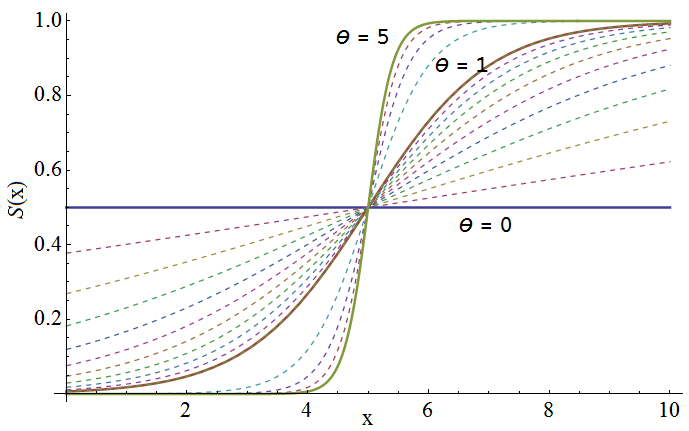
\includegraphics[width=\columnwidth]{../figures/sigmoid1.png}
\centering\caption{}\label{fig:sigmoid}
\end{figure}

A similar argument can be made in the case where agents have unreliable communication as well as noisy sensor measurements. We instead propose the use of a continuous, sigmoid threshold function for computing collaboration probability. The sigmoid function we use is commonly referred to as the \emph{logistic} function and is mathematically defined as,
\begin{equation}\label{eq:sig}
	\sig(\estg, \estt, \theta) = \frac{1}{1 + e^{\theta(\estt - \estg)}}
\end{equation}
Here, the term $\theta$ is referred to as the sigmoid slope parameter as it controls the slope of the curve at $\sig(\cdot) = 0.5$, as seen in Fig.~\ref{fig:sigmoid}. 
\begin{equation}
	\sig(\estg, \estt, \theta) =  \left\{
	\begin{array}{ll}
		0.5 & : \theta = 0\\ 
		P_{yes}(\estt,\estg) & : \theta \to \infty
	\end{array}\right.
\end{equation}
When $\theta = 0$, the sigmoid curve becomes the straight line $\sig(\estg, \estt, 0) = 0.5$ and as $\theta \to \infty$, Eq.~\ref{eq:sig} begins to resemble the step function seen in Eq.~\ref{eq:step}.

\section{Experiment Setup}\label{sec:expsetup}
We ran collaborative task completion experiments with the \emph{Droplet} swarm robot platform to validate results presented in the previous section. The experiment employs they robots' overhead RGB sensors to simulate a fire that is projected down onto the arena using a standard off-the-shelf projector. The goal of the experiment is to have the robots collaboratively put out these projected fires by congregating at the perimeter of the fire and turning on their blue LEDs together. The projected fires increase in size and intensity (indicated by changing color from the red to the yellow spectrum) with time.



\section{Experimental Results}\label{sec:expresults}




\section{Discussion}\label{sec:disc}




\section{Conclusion}\label{sec:conc}




%%%%%%%%%%%%%%%%%%%%%%%%%%%%%%%%%%%%%%%%%%%%%%%%%%%%%%%%%%%%%%%%%%%%%%%%%%%%%%%%
%%%%%%%%%   The Bibliography, if any   %%%%%%%%%
\bibliographystyle{IEEEtran}		% or "siam", or "alpha", etc.
\bibliography{../refworks}
\end{document}
